
\documentclass[pdflatex,sn-mathphys-num]{sn-jnl}% Math and Physical Sciences Numbered Reference \usepackage{graphicx}%
\usepackage{multirow}%
\usepackage{amsmath,amssymb,amsfonts}%
\usepackage{ragged2e} % Para justificación
\usepackage{amsthm}%
\usepackage{tikz}
\usetikzlibrary{positioning, shapes.geometric}
\usepackage{mathrsfs}%
\usepackage[title]{appendix}%
\usepackage{xcolor}%
\usepackage{textcomp}%
\usepackage{manyfoot}%
\usepackage{booktabs}%
\usepackage{algorithm}%
\usepackage{algorithmicx}%
\usepackage{algpseudocode}%
\usepackage{listings}%
\usepackage{pdfpages}
%%%%
\usepackage{hyperref}
\usepackage{fontawesome5} % For the GitHub icon

%% as per the requirement new theorem styles can be included as shown below
\theoremstyle{thmstyleone}%
\newtheorem{theorem}{Theorem}%  meant for continuous numbers
%%\newtheorem{theorem}{Theorem}[section]% meant for sectionwise numbers
%% optional argument [theorem] produces theorem numbering sequence instead of independent numbers for Proposition
\newtheorem{proposition}[theorem]{Proposition}% 
%%\newtheorem{proposition}{Proposition}% to get separate numbers for theorem and proposition etc.

\theoremstyle{thmstyletwo}%
\newtheorem{example}{Example}%
\newtheorem{remark}{Remark}%

\theoremstyle{thmstylethree}%
\newtheorem{definition}{Definition}%

\raggedbottom
%%\unnumbered% uncomment this for unnumbered level heads

\begin{document}

\title[Article Title]{Multiplicador Booth Wallace}



\author*[1,2]{\fnm{Contreras R} \sur{Orlando}}\email{\{al348390,al307630\}@edu.uaa.mx}
\author*[1,2]{\fnm{Garcia B} \sur{Iker}}
\equalcont{Ambos autores contribuyeron de forma equitativa a este trabajo.}


\affil[3]{\orgdiv{Departamento de Sistemas Electrónicos}, \orgname{UAA}, \orgaddress{\street{Av. Universidad 940}, \city{Aguascalientes}, \postcode{20131}, \state{Aguascalientes}, \country{México}}}


%%==================================%%
%% Sample for unstructured abstract %%
%%==================================%%

\abstract{El presente documento busca implementar la multiplicación de la forma más efectiva, para ello se usara el codificamiento de Booth en Radix 2, e implementar la suma mediante Carry save's siguiendo la estructura del Arbol de Wallace}

%%================================%%
%% Sample for structured abstract %%
%%================================%%

\keywords{VHDL, FPGA, Booth, Multiplicador, Carry Save,  Multiplicador con Signo}


\maketitle
\section{Introducción}\label{sec1}
Este multiplicador de 8x8 combina la eficiencia del algoritmo de Booth para la codificación de los operandos con el uso de sumadores en paralelo tipo Wallace Tree para la reducción rápida de productos parciales. Esta arquitectura permite optimizar la multiplicación de números con signo al reducir la cantidad de operaciones necesarias y mejorar el rendimiento general del sistema. Su diseño representa una aproximación avanzada en la implementación de multiplicadores aritméticos dentro del ámbito del diseño digital. \\

\justify

La multiplicación eficiente es un componente esencial en una amplia gama de aplicaciones como procesamiento digital de señales, visión por computadora, aprendizaje automático y sistemas embebidos. En estos casos, es necesario ejecutar operaciones aritméticas complejas con alta velocidad y precisión, especialmente cuando se trata de datos en formato binario con signo. En este sentido, el multiplicador 8x8 basado en la técnica Booth-Wallace se presenta como una solución eficiente y escalable para tareas de procesamiento intensivo en hardware digital. \\
\section{Metodología}\label{sec1}
\subsection{Booth}
Para poder implementar este codificado fue necesario manejar las entradas de diferente forma; en multiplicadores pasados hacíamos directamente el producto multiplicando cada término, en este no, lo que se hará es tomar un vector como el de control y otro como el que se irá sumando/restando según sea el caso, como se puede apreciar en \ref{tab:booth_cases}. Cabe hacer mención que para restar el valor deberemos aplicar complemento a dos extendiendo a 16 bits siendo nuestra entrada de 8 bits. 

El método de Booth establece que debe analizarse en bits al vector de control, en este caso para el RADIX-2 se analizará por pares, además de esto, es necesario añadir 2 bits extra con el valor de 0, uno al inicio y otro al final, esto para considerar esos dos casos. Se contará con varios acumuladores, que serán nuestros productos parciales. 

Después de cada operación se deberá ir recortando el bit y rellenarse con 0's, para poder apreciar esto de una mejor forma se puede ver en el siguiente esquemático, siendo la estructura \textit{generate} con valores de 0 a 8, se puede ver como cada valor se irá almacenando en una memoria/\textit{array}. Donde cada uno será un vector de tamaño de 16 bits, es decir,se tendrá un vector de vectores, siendo el tamaño de la memoria de 6 vectores. En la figura \ref{fig:DSNBooth} se puede apreciar la arquitectura construida.
\begin{table}[h!]
\centering
\caption{Casos del algoritmo de Booth radix-2}
\begin{tabular}{cccl}
\toprule
$Q_1$ & $Q_0$ & Acción            & Operación         \\
\midrule
0     & 0     & Nada              & $A= \text{x}0000$    \\
0     & 1     & Sumar $M$         & $A = M$      \\
1     & 0     & Restar $M$        & $A =- M$     \\
1     & 1     & Nada              & $A= \text{x}0000$   \\
\bottomrule
\end{tabular}
\label{tab:booth_cases}
\end{table}

\begin{figure}[H]
    \centering
    \includegraphics[scale=0.25]{2_examen/BoothFigma.png}
    \caption{Diseño de Booth}
    \label{fig:DSNBooth}
\end{figure}
\subsection{Arbol de Wallace}
Una vez teniendo nuestros productos parciales, procederemos a sumarlos. Como se explicó previamente, se creó un vector llamado PP donde se almacenan vectores, siendo cada vector un Producto Parcial. Para poder sumar de forma efectiva implementaremos el carry save que prácticamente son half adder concatenados sin propagar el carry entre ellos, cada bloque de Carry Save tiene 3 entradas, y tendrá dos salidas, la salida para Carry y la salida para la suma, en el último bloque se usará un propagador de carry, puede usarse un full adder sin problema, se utilizó un carry look ahead (CLA) como optimización de tiempos. En la arquitectura se instanciaron 7 bloques, se puede apreciar toda la arquitectura en la figura \ref{fig:Main}.
\begin{figure}[H]
    \centering
    
\includegraphics[scale=0.25]{2_examen/MainArc.png}
    \caption{Arquitectura completa}
    \label{fig:Main}
\end{figure}





\section{Resultados}\label{sec2}

Se puede observar en la simulación como los valores de la multplicacion son correctos y el signo de salida esta invertido, esto es ya que el led de salida de signo que usamos es un led interno de la tang nano y prende con 0 en ves de con unos.

\begin{figure}[H]
    \centering
    \includegraphics[width=1\linewidth]{2_examen/tb.png}
    \caption{Testbench realizado por Xilinx}
    \label{fig:enter-label}
\end{figure}

\begin{figure}[h]
    \centering
    \includegraphics[width=0.70\linewidth]{2_examen/tang.png}
    \caption{Circuito Armado}
    \label{fig:enter-label}
\end{figure}

\begin{figure}[h]
    \centering
    \includegraphics[width=0.55\linewidth]{2_examen/4.png}
    \caption{Summary report generated by Xilinx}
    \label{fig:enter-label}
\end{figure}
\newpage

\section{Conclusiones}\label{sec4}
Lo más desafiante de esta práctica fue investigar y comprender el funcionamiento del algoritmo de Booth y los carry-save adders de Wallace, así como su correcta implementación en código, asegurándonos de que no existieran casos que pudieran fallar. Uno de los principales retos surgió al manejar el valor de entrada FF, ya que en ese caso solo se generaba un producto parcial distinto de cero, lo que indicaba un comportamiento incorrecto. La solución consistió en agregar un bit adicional al final, lo que permitió que el algoritmo funcionara correctamente y resolviera el problema.

\section{Anexos} % Aqui poner los RTL

Esto es la parte más importante de los RTL, si se gusta observar con mayor detalle, los PDFs estarán en el documento adjunto. Asimismo se podrá observar el código actualizado en:
\href{https://github.com/DasRexyr/HDL-ART}{\faGithub\ GitHub Repository}

\begin{figure}[H]
    \centering
    \includegraphics[width=0.5\linewidth]{2_examen/1.png}
    \caption{RTL del Componente principal}
    \label{fig:enter-label}
\end{figure}

\begin{figure}[H]
    \centering
    \includegraphics[width=0.5\linewidth]{2_examen/2.png}
    \caption{RTL del CSA}
    \label{fig:enter-label}
\end{figure}

\begin{figure}[H]
    \centering
    \includegraphics[width=0.5\linewidth]{2_examen/3.png}
    \caption{RTL del Componente CLA}
    \label{fig:enter-label}
\end{figure}

\begin{figure}[H]
    \centering
    \includegraphics[width=0.5\linewidth]{p6/SQ3.png}
    \caption{RTL del Componente Complemento a 2}
    \label{fig:enter-label}
\end{figure}

\begin{figure}[h!]
\centering
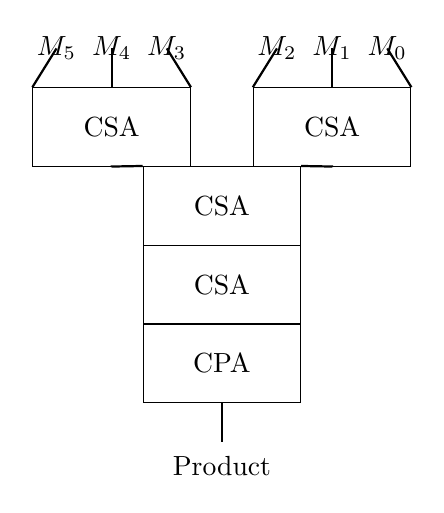
\begin{tikzpicture}[
  block/.style={rectangle, draw, minimum width=2cm, minimum height=1cm, text centered},
  line/.style={draw, thick}
]

% Bit labels
\node at (-2.1,4) {$M_5$};
\node at (-1.4,4) {$M_4$};
\node at (-0.7,4) {$M_3$};
\node at (0.7,4) {$M_2$};
\node at (1.4,4) {$M_1$};
\node at (2.1,4) {$M_0$};

% CSA Layers
\node[block] (csa1a) at (-1.4,3) {CSA};
\node[block] (csa1b) at (1.4,3) {CSA};
\node[block] (csa2) at (0,2) {CSA};
\node[block] (csa3) at (0,1) {CSA};
\node[block] (cpa) at (0,0) {CPA};

% Connections from inputs
\draw[line] (-2.1,4) -- (csa1a.north west);
\draw[line] (-1.4,4) -- (csa1a.north);
\draw[line] (-0.7,4) -- (csa1a.north east);

\draw[line] (0.7,4) -- (csa1b.north west);
\draw[line] (1.4,4) -- (csa1b.north);
\draw[line] (2.1,4) -- (csa1b.north east);

% CSA connections
\draw[line] (csa1a.south) -- (-1.4,2.5) -- (csa2.north west);
\draw[line] (csa1b.south) -- (1.4,2.5) -- (csa2.north east);

\draw[line] (csa2.south) -- (csa3.north);
\draw[line] (csa3.south) -- (cpa.north);

% Output
\draw[line] (cpa.south) -- (0,-1);
\node at (0,-1.3) {Product};

\end{tikzpicture}
\caption{Wallace-tree multiplier core (6-bit example)}
\end{figure}


\end{document}
